\section{Results \& Discussion}
This section is dedicated to the description of the results obtaine from several experiments based on the above algorithm. We first describe the performance of the algorithm simulated in Matlab using synthetic optic-flow measurements. Then, we consider comparing estimates given by the algorithm to the "ground truth" obtained form a high-precision motion capture system.

\subsection{Simulation on Matlab}
The algorithm described in the previous section was first implemented in C to work on the embedded hardware. However, in order to verify its efficiency the code was translated into Matlab as faithfully as possible to the code used on the optic-flow sensor. Thus, the inner-workings of the key functions (e.g. back-projection, voting, etc.) were kept the same and did not make use of equivalent Matlab built-in functions. 

The sampling pixels were chosen identical to the ones used on the vision system, i.e. 81 pixels were uniformly distributed on a rectangular grid of 160x120 (corresponding to the camera resolution). They are then back-projected onto the unit sphere using the method detailed above. The optic-flow measurements are generated using the first-order approximation (\ref{equ:opticflow}). Outliers are simulated by adding randomly generated tangent vectors to a subset of the optic-flow vectors. The resulting optic-flow vectors are derotated and the normal vectors corresponding the great circles are computed in the same way as in the C implementatin. Finally, voting is performed and the best estimate is found and compared to the actual direction of motion set by the user.

We first consider a single refinement stage in the estimation of the direction of translation. Then, 3 more stages are added as stated in the previous section. The parameters that were used are detailed in Table~\ref{tab:simParam}.
\begin{table}[h]
\centering
\begin{tabular}{c|c|c|c}
Velocity ($V$) & Angular rate ($w$) & Depth of scene ($D$) & Samples ($P$)\\
\hline
$[0.56, 0.42, 0.13]$ & $[0, \pi/3, \pi/5]$ & $50\cdot10^{-2}$ & 81\\
\end{tabular}
\caption{\textbf{Simulation parameters} - The velocity and angular velocity were divided by the frequency of the camera (200Hz) to emulate real optic-flow computation\label{tab:simParam}}
\end{table}
Figures~\ref{fig:simOpticFlow}-\ref{fig:simDerotation} depicts respectively the sampling points and the optic-flow vectors, the outliers and the final set of vectors after derotation.

\begin{figure}
\centering
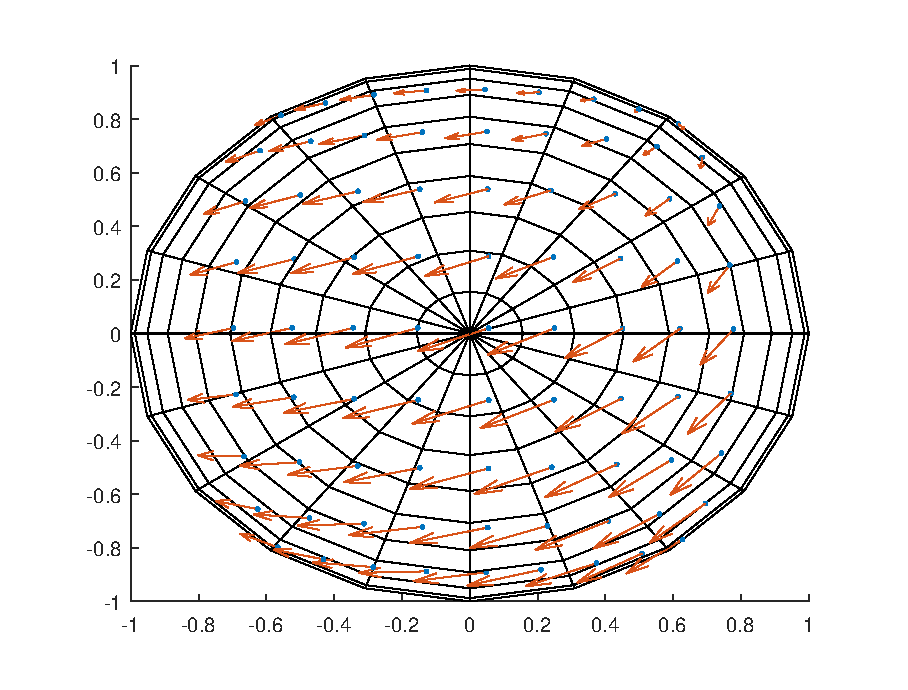
\includegraphics[width=0.6\linewidth]{images/matlab/simOpticFlow.eps}
\caption{\textbf{Generated sampling points and optic-flow vectors} - Synthesized using the first-order approximation and the parameters detailed in Table~\ref{tab:simParam}}
\label{fig:simOpticFlow}
\end{figure}

\begin{figure}
\centering
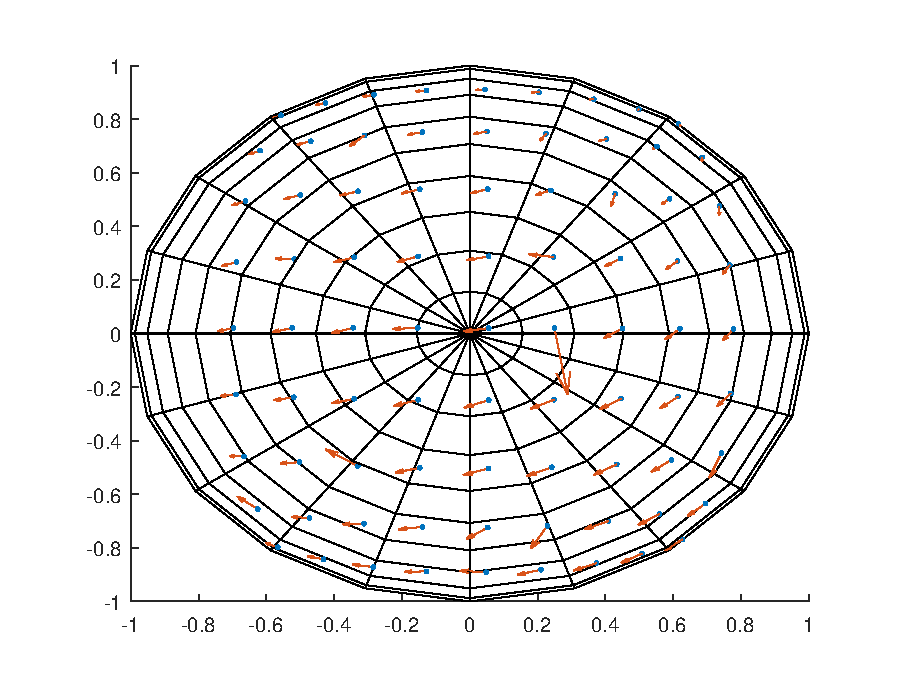
\includegraphics[width=0.6\linewidth]{images/matlab/simOutliers.eps}
\caption{\textbf{Generated outliers} - Synthesized using the first-order approximation and the parameters detailed in Table~\ref{tab:simParam} and additional randomly generated tangent vectors}
\label{fig:simOutliers}
\end{figure}

\begin{figure}
\centering
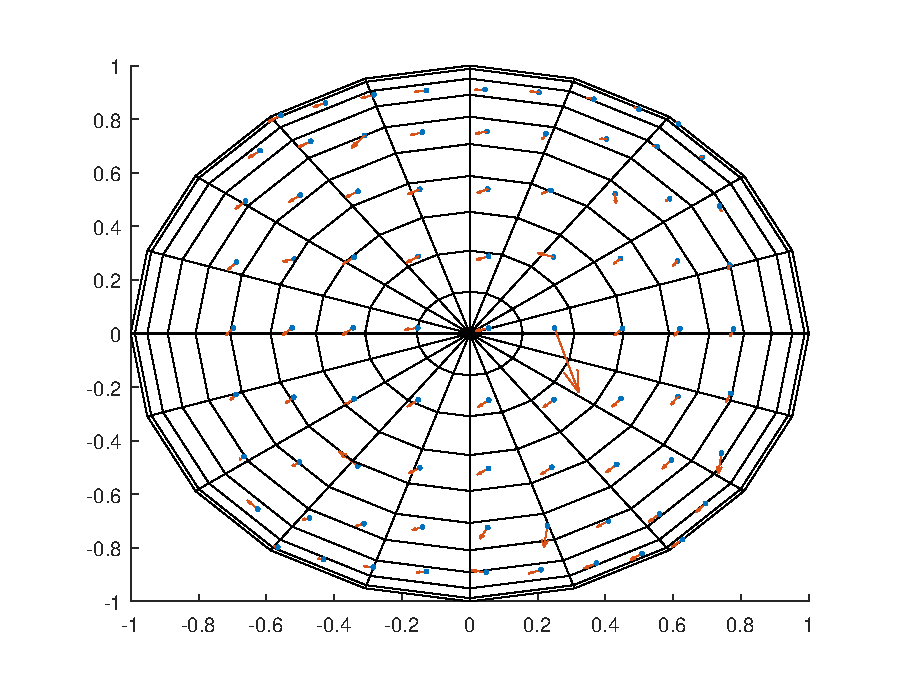
\includegraphics[width=0.6\linewidth]{images/matlab/simDerotation.eps}
\caption{\textbf{Derotated optic-flow vectors} - Synthesized using the first-order approximation and the parameters detailed in Table~\ref{tab:simParam} and additional randomly generated tangent vectors}
\label{fig:simDerotation}
\end{figure}

Both versions of the algorithm (Table~\ref{tab:votingBins}) are applied on synthetic optic-flow field with varying propotions of outliers. These outliers are randomly generated using the same seed for a fair comparision between the two. The results are averaged over 100 runs and correspond to the values of the dot products between the estimated and real directions of motion (which are unit vectors). From Table~\ref{tab:simResults}, it can be inferred that using fewer voting stages makes the algorithm less slightly less sensible to outliers (at the expense of a significantly higher computational cost). Indeed, more stages means that outliers may still be present in intermediary stages and influence the estimate, all the more so when their proportion is greater than the one of the inliers. As the latter case may be rare in reality or avoided through the use of a quality factor on the optic-flow measurements, one may consider finding a trade-off between the number of stages (i.e. lowering the runtime) and the number of bins in each stage (i.e. the robustness and accuracy).

\begin{table}
\centering
\begin{tabular}{|c|c|c|c|c|}
\hline
\multirow{2}{*}{Stages} & \multirow{2}{*}{Accuracy} & \multicolumn{3}{c|}{Proportion of outliers}\\
\cline{3-5}
  & & 25\% & 50\% & 75\% \\
\hline
\multirow{2}{*}{2}  & Mean & 0.999782 & 0.999782 & 0.850839 \\
\cline{2-5}
& Std. dev. & 0.000000 & 0.000000 & 0.320995 \\
\hline
\multirow{2}{*}{5}  & Mean & 0.999913 & -0.999180 & 0.849634 \\
\cline{2-5}
& Std. dev. & 0.000000 & 0.002944 & 0.322923 \\
\hline
\end{tabular}
\caption{\textbf{Influence of outliers on estiamte} - The dot products of the estimated and real directions of motion are averaged over 100 runs with various proportions of outliers\label{tab:simResults}}
\end{table}


\subsection{Experiments with motion capture}
\subsubsection{Setup}
Experiments were conducted moving the camera by hand in a synthetic environment (i.e. textured walls) while recording its full displacement thanks to a motion capture system. These experiments were meant to assess the performance of the method described in Section II for estimating the direction of motion but may not be representative of its actual robustness under all conditions (different illumination, environment textures, etc.).

The optic-flow sensor consists in a PX4Flow board which integrates a 168MHz Cortex M4F CPU, a 3-axis rate gyro, a sonar, and the actual machine vision sensor. The biases and noise of the gyro are compensated by averaging and low-pass filtering and the scaling factor for derotation is stored in memory. A Sunex DSL215 fisheye lens is mounted on the board, allowing for a 185 degrees diagonal field of view in full frame format. The camera image is 160x120 pixel wide and sampled at 200Hz. All computations are performed on the chip and the estimates of the direction of motion are sent via USB and logged through QGroundControl (v.2.7).

We sample up to 117 optic-flow at each iteration (~160Hz), the latter of which are estimated using the Lucas-Kanade method on 10x10 binned image (patch). The vantage points corresponding to the optic-flow measurements are evenly distributed on the (rectangular) camera image. Although evenly-distributing points on the unit sphere was first considered - as it allows to uniformly sample the field of view -, this latter solution would imply overlapping in the binned image, thus increasing the statistical probability of encountering outliers. To cope with this issue, one may choose to adapt the size of the neighborhood (image patches) used in the optic-flow computation as proposed in \cite{adapted_neighborhood}.

% Describe optic-flow sensor board (chip + gyroscope)
% Describe lens (sunex)
% Describe sampling directions and number (and why)
% Describe image caching (built in function) and gyroscope sampling (same)
% Describe the remaining elements (sampling rate, algorithm run on chip)

% Descripton: PX4Flow is an optical flow smart camera (it provides the image for setup purposes, but it not designed to capture images like a webcam). It has a native resolution of 752�480 pixels and calculates optical flow on a 4x binned and cropped area at 400 Hz, giving it a very high light sensitivity. Unlike many mouse sensors, it also works indoors and in low outdoor light conditions without the need for an illumination LED. It can be freely reprogrammed to do any other basic, efficient low-level computer vision task.

% 168 MHz Cortex M4F CPU (128 + 64 KB RAM)
% 752�480 MT9V034 image sensor, L3GD20 3D Gyro
% 16 mm M12 lens (IR block filter)
% Size 45.5 mm x 35mm
% Power consumption 115mA / 5V

% \begin{itemize}
% \item MT9V034 machine vision CMOS sensor with global shutter
% \item Optical flow processing at 4�4 binned image at 400 Hz
% \item Superior light sensitivity with 24�24 �m super-pixels
% \item Onboard 16bit gyroscope up to 2000�/s and 780 Hz update rate, default high precision-mode at 500�/s
% \item Onboard sonar input and mount for Maxbotix sonar sensors. (HRLV-EZ4 recommended, SparkFun Product Link)
% \item USB bootloader
% \item USB serial up to 921600 baud (including live camera view with QGroundControl)
% \item USB power option
% \end{itemize}

% High Resolution Fisheye Lens:

% The DSL215 lens is a multi-megapixel miniature fisheye lens that achieves a 185 degree diagonal field of view on 1/4" format (full frame):
% Specifications:

% \begin{itemize}
% 	\item Imager format: 1/4"
% 	\item Focal length: 1.55mm (enables good low light performance)
% 	\item Relative aperture: F/2.0
% 	\item Image circle: 4.7mm
% 	\item Field of view: 138� at 3.6mm image circle / 185� at 4.7mm image circle
% \end{itemize}

% The optic-flow measurements are sampled at 200Hz while the full direction of motion estimation algorithm is run on the optic-flow sensor chip. 
\begin{figure}[h]
\centering
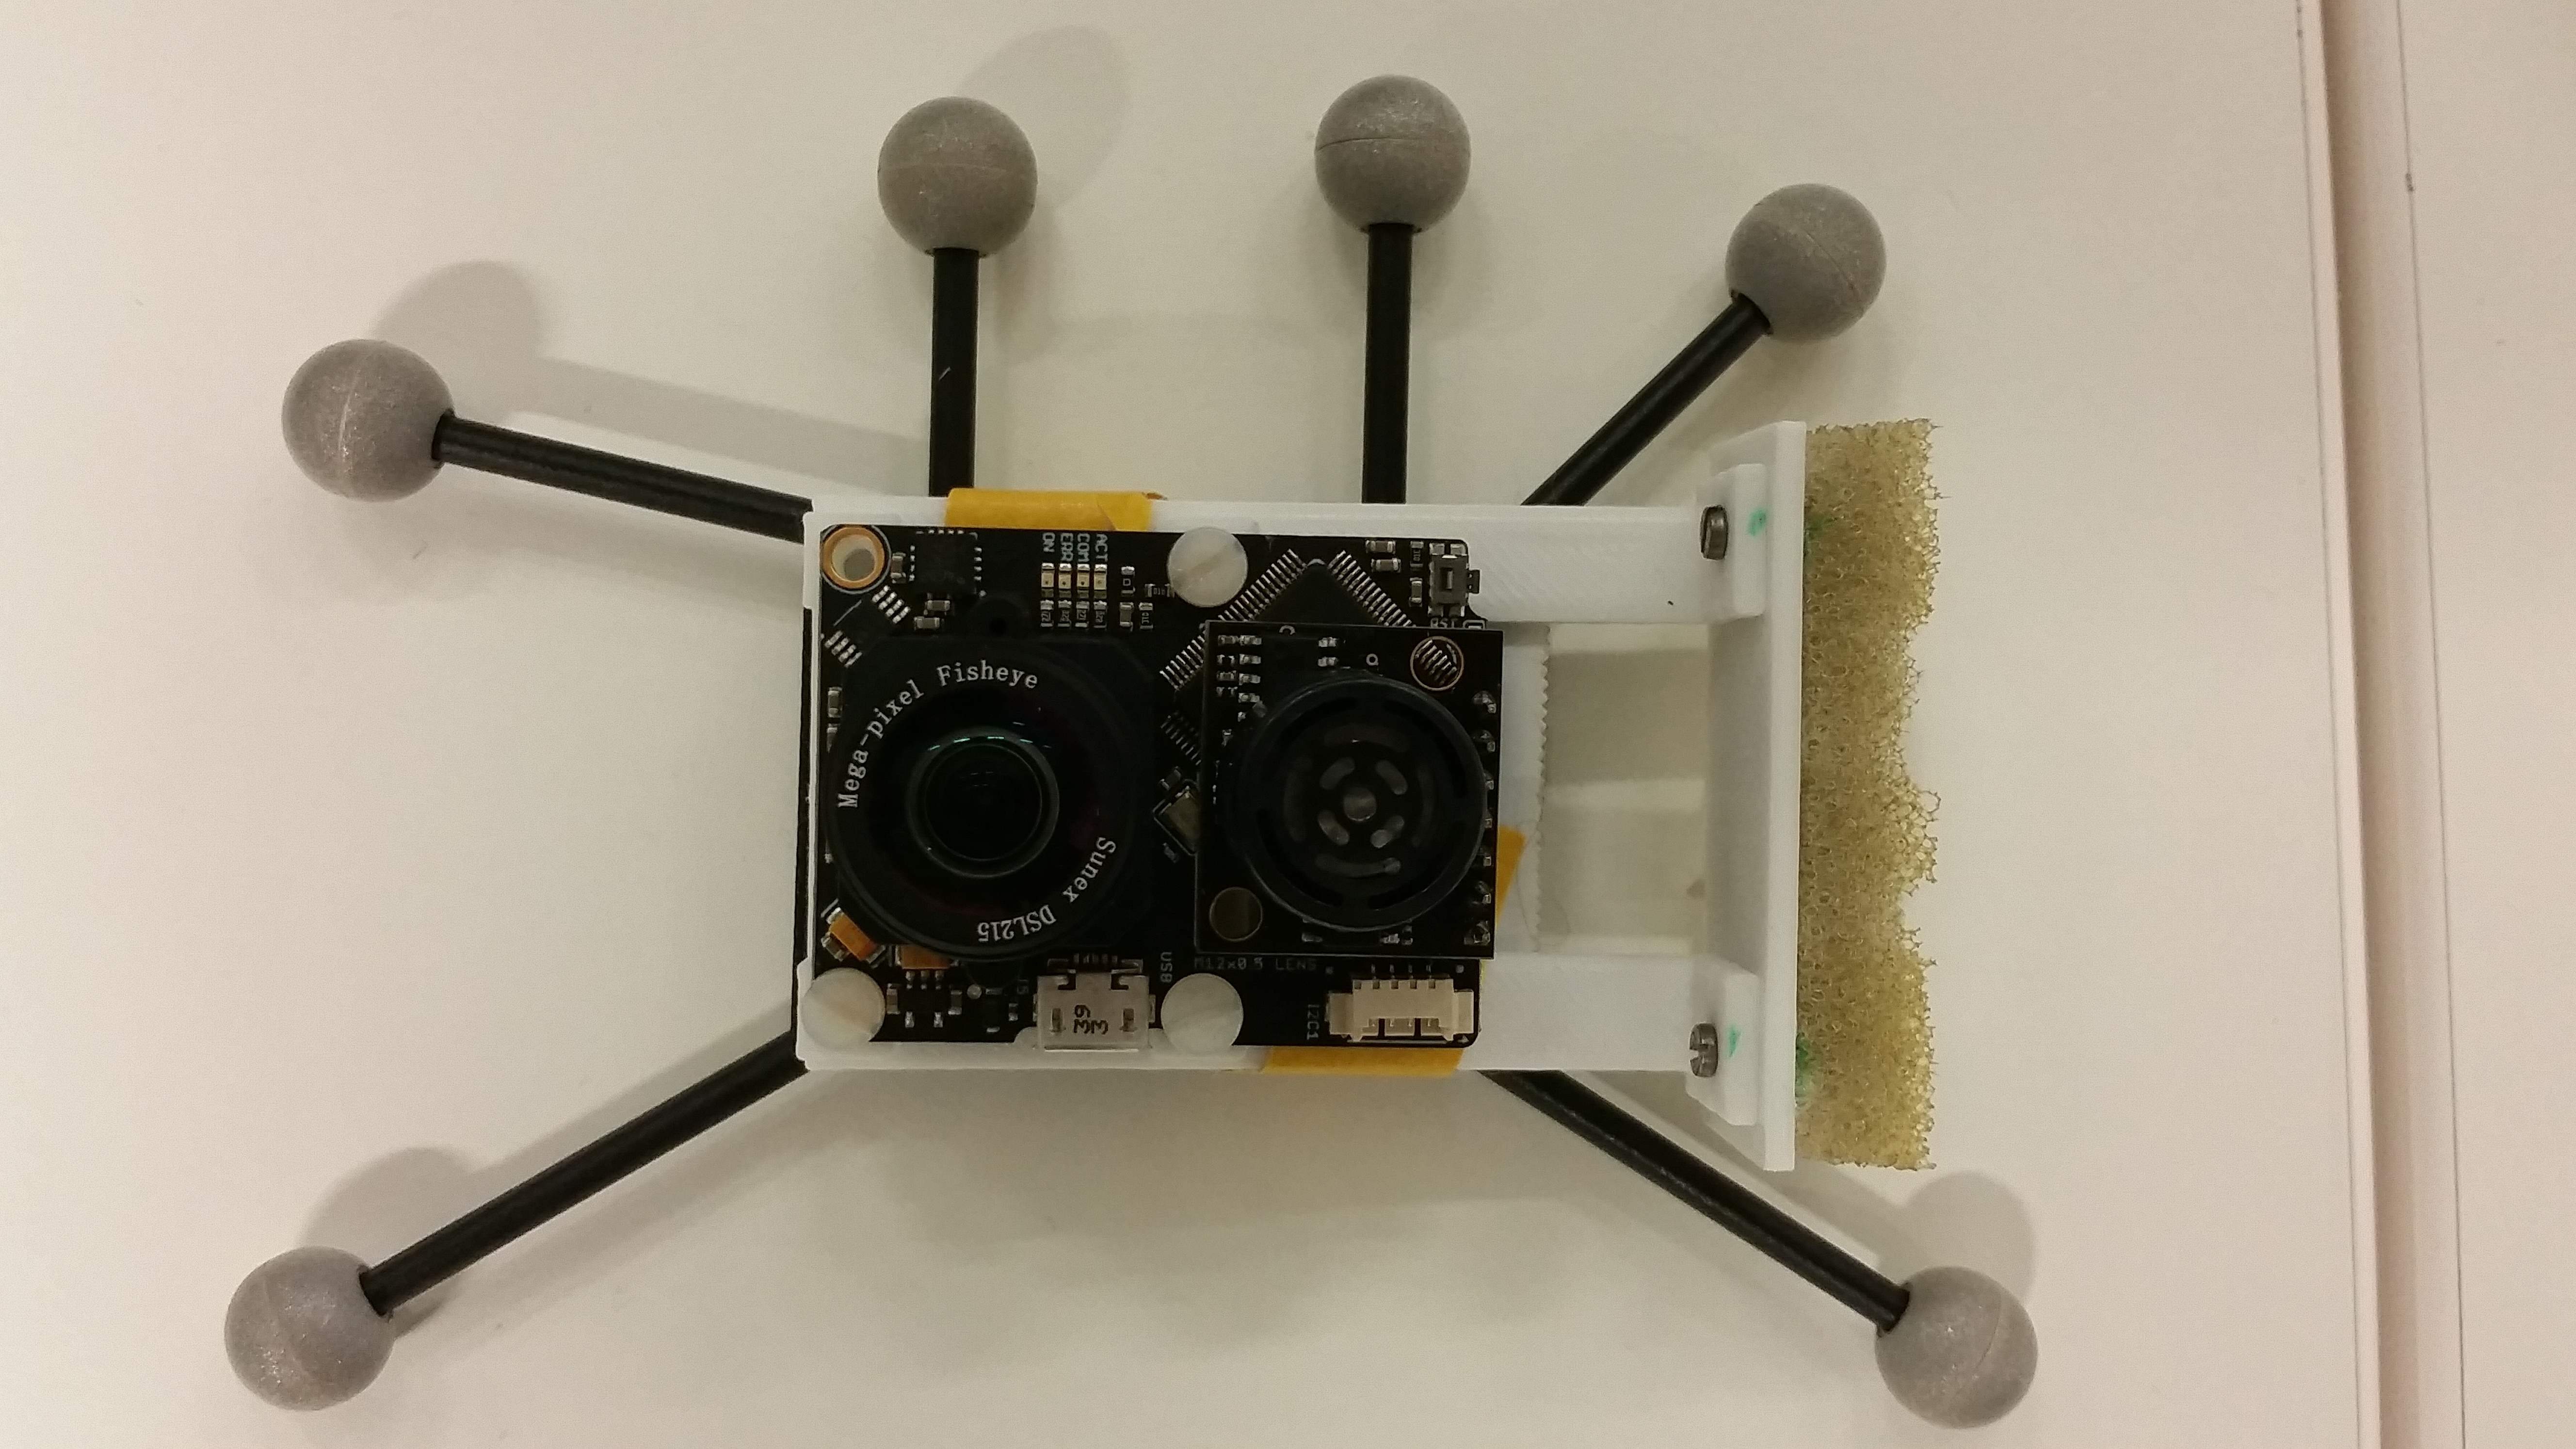
\includegraphics[width = 0.5\linewidth]{images/moCapFrame.jpg}
\caption{\textbf{Optic-flow sensor mounted on its motion capture frame} - The frame is equipped with 5 passive markers attached at known positions to obtain 3D position and orientation of the rigid body out of the 21 IR cameras.}
\label{fig:motionCapture}
\end{figure}

Experiments were performed using an OptiTrack motion capture system which high precision allowed to estimate the ground truth measurements. The optic-flow sensor was mounted on a frame equipped with 5 markers (coated with a reflective material) attached at known positions to obtain the three-dimensional position and orientation of the rigid body (Fig.~\ref{fig:motionCapture}). The motion of the camera was recorded at 250Hz using a set of 21 IR cameras. The measured orientation are differentiated so as to obtain the angular rates of the rigid body, which are compared to the gyroscopes measurements for synchronization purposes (convolution).


Motion capture using passive markers requires the emission of IR lights that are sensed by the camera due to its small size. Due to the frequency at which these articial lights were emitted (250Hz), the ambiant illumination as seen by the camera (200Hz) typically changed every 150ms inducing an automatic calibration of the luminosity, which requires extra 5ms before new readings are sampled. Although this setup was kept due to time constraints, this issue could be avoided by switching of IR lights and using active markers (i.e. a set IR LEDs).

\subsubsection{Results}
The experiments were performed using the algorithm detailed above with 5 stages refinements. Two different number of samples were tested; the first one being 81, which typically enables a runtime of 5.3ms, and the second one being 117, which runs at approximately 160Hz.

As the measurements obtained from the optic-flow sensor and the motion capture system were not started simultaneously, we had to synchronize them afterwards. To ease up the process, we performed a recognizable motion that involved the gyroscope of the camera. Indeed, the gyroscope measurements are typically much less noisy than the optic-flow data. Hence, the angular rates measured by the optic-flow sensor were stored and compared to the estimates of the rates inferred from the motion capture system. The derivatives of the quaternions given by OptiTrack were computed using the three points rule, which typically allows for a better estimate. They were then converted from global to local (camera) coordinates. The synchronization was realized manually as recognizable points were easily located. Note that since the two systems exhibit different refresh rates, the values of the camera gyroscope were interpolated using a standard linear regressor between each datapoint. Finally, one may consider smoothing the data (e.g. using a gaussian window) although this was not required for synchronizing the signals in our case. Some results of the synchronization process are shown in Figures~\ref{fig:mocapGyro81}-\ref{fig:mocapGyro117}.

\begin{figure}
\centering
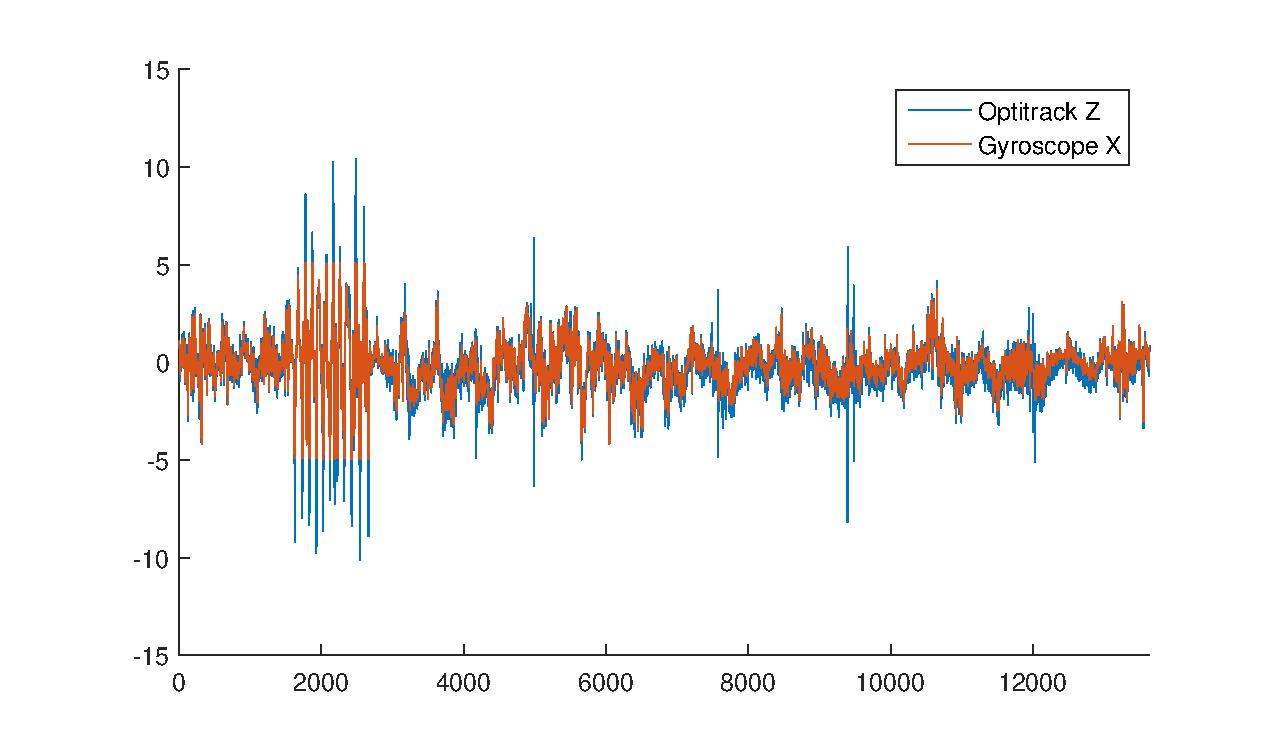
\includegraphics[width = 0.8\linewidth]{images/matlab/mocapGyro81}
\caption{\textbf{Synchronized signals from camera and optitrack} - The signals were synchronized manually using recognizable features. The axes of the optitrack were circularly permutated so as to correspond to the ones used in the camera frame. The horizontal axis correspond to the index of the frame (~5ms)}
\label{fig:mocapGyro81}
\end{figure}

\begin{figure}
\centering
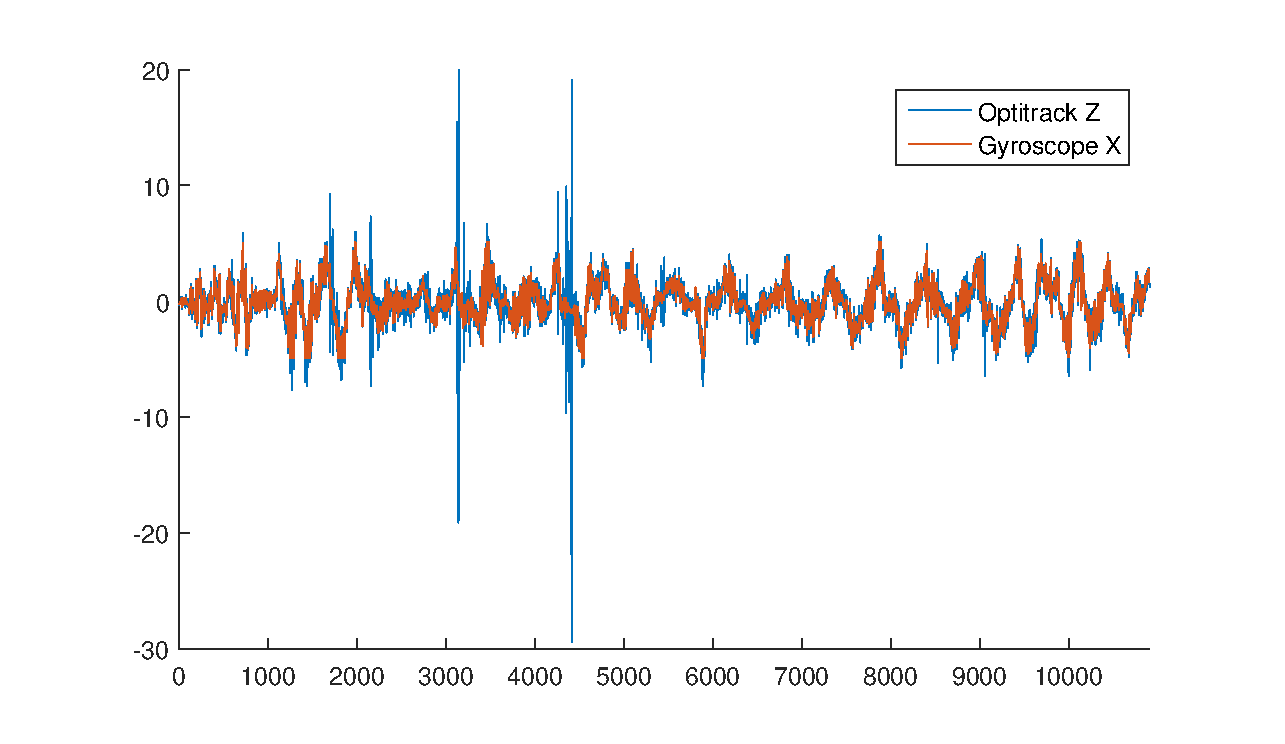
\includegraphics[width = 0.8\linewidth]{images/matlab/mocapGyro117}
\caption{\textbf{Synchronized signals from camera and optitrack} - The signals were synchronized manually using recognizable features. The axes of the optitrack were circularly permutated so as to correspond to the ones used in the camera frame. The horizontal axis correspond to the index of the frame (~5ms)}
\label{fig:mocapGyro117}
\end{figure}

As it can be seen on Figures~\ref{fig:mocapGyro81}-\ref{fig:mocapGyro117}, both signals display comparable accuracy although some spikes are visible on the OptiTrack estimates. These spikes may be due to markers being lost by the motion capture system (thus inducing very fast changes in the orientation of the rigid body).

The direction of motion was estimated from motion capture outputs using the 3 point rule on the 3D position. This so-called "ground-truth" is compared to the optic-flow sensor estimates. The raw meaasurements obtained for 81 viewing directions are shown in Figure~\ref{fig:mocapPos81}. As it can be seen on the figure, the signals are display very fast oscillations that can hardly be considered similar although they seem to follow a same "trend".

\begin{figure}
\centering
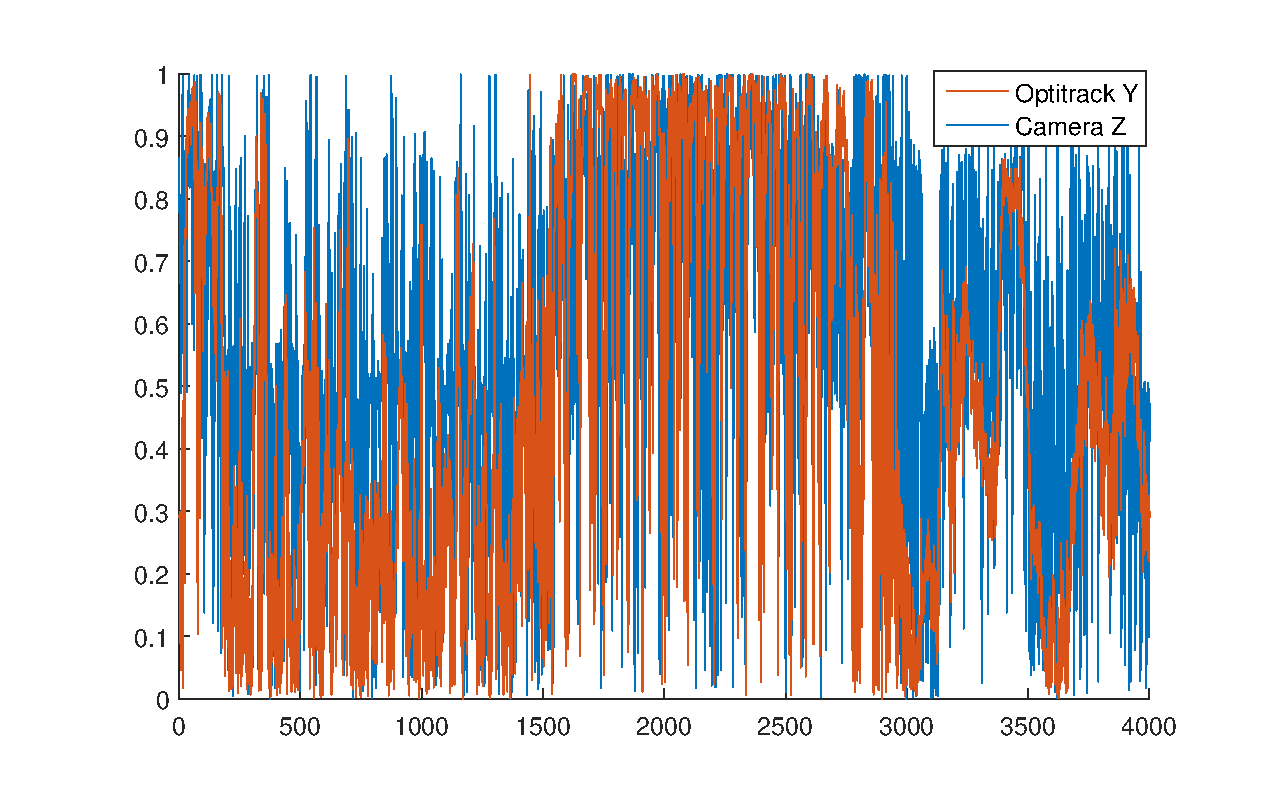
\includegraphics[width = \linewidth]{images/matlab/mocapPos81}
\caption{\textbf{Comparison of optic-flow sensor estimate with "ground-truth"} - The horizontal axis correspond to the index of the frame (~5ms) \label{fig:mocapPos81}}
\end{figure}

To cope with the high oscillations, we smooth the data using gaussian windows. The first one, which is equivalent to a $\sigma=4ms$, yields the graph shown in Figure~\ref{fig:mocapPos81_sig4}. The result shows a good correlation between the two signal although the optic-flow sensor estimate still exhibit high error when compared to the motion capture measurements. By increasing the width of the gaussian window ($\sigma = 20ms$), the estimates still appear correlated, meaning that our method is correct. 

However, in all cases, the values are far from the "ground truth". Whether the changing ambiant lighting has influenced the estimation of the estimation of the direction of motion remains an open question.

\begin{figure}[t]
\centering
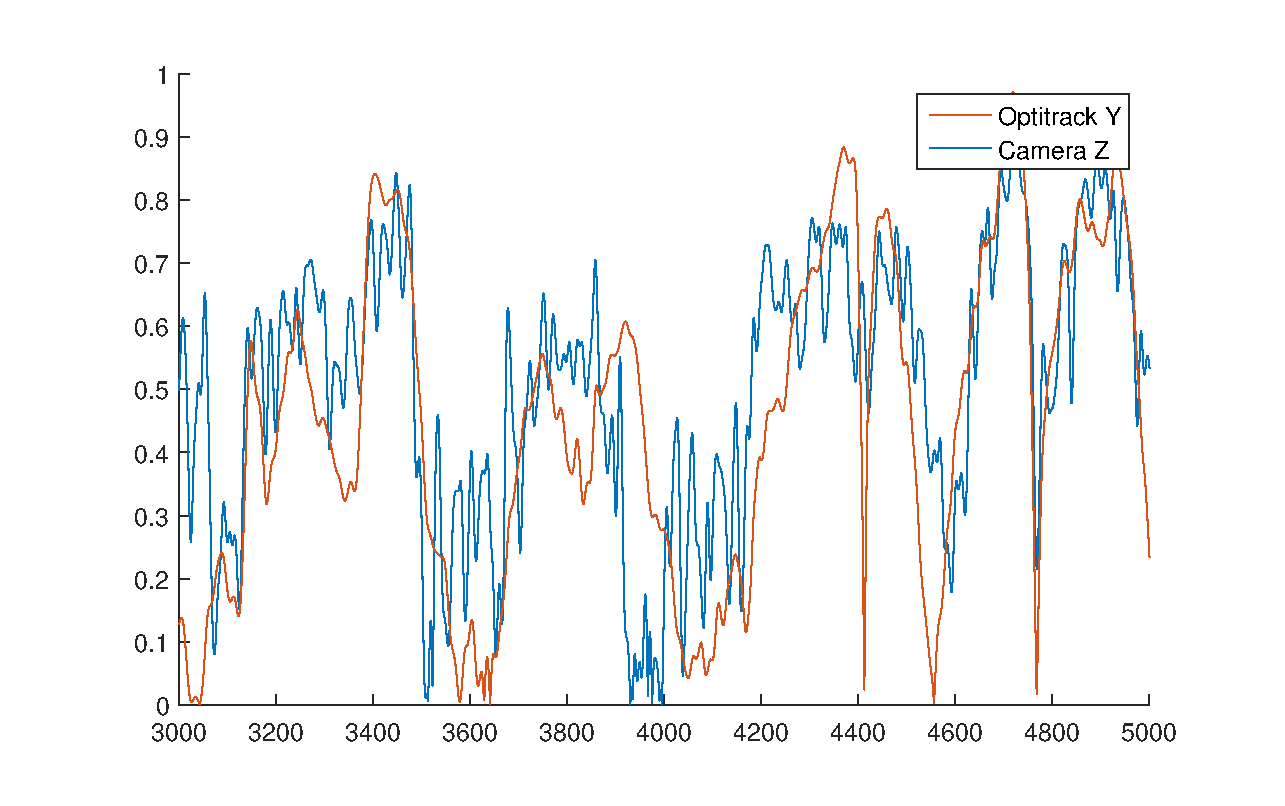
\includegraphics[width = \linewidth]{images/matlab/mocapPos81_sig4}
\caption{\textbf{Comparison of optic-flow sensor estimate with "ground-truth" (cont'd)} - A gaussian window ($\sigma = 4ms$) was applied. The horizontal axis correspond to the index of the frame (~5ms) \label{fig:mocapPos81_sig4}}
\end{figure}

\begin{figure}[b]
\centering
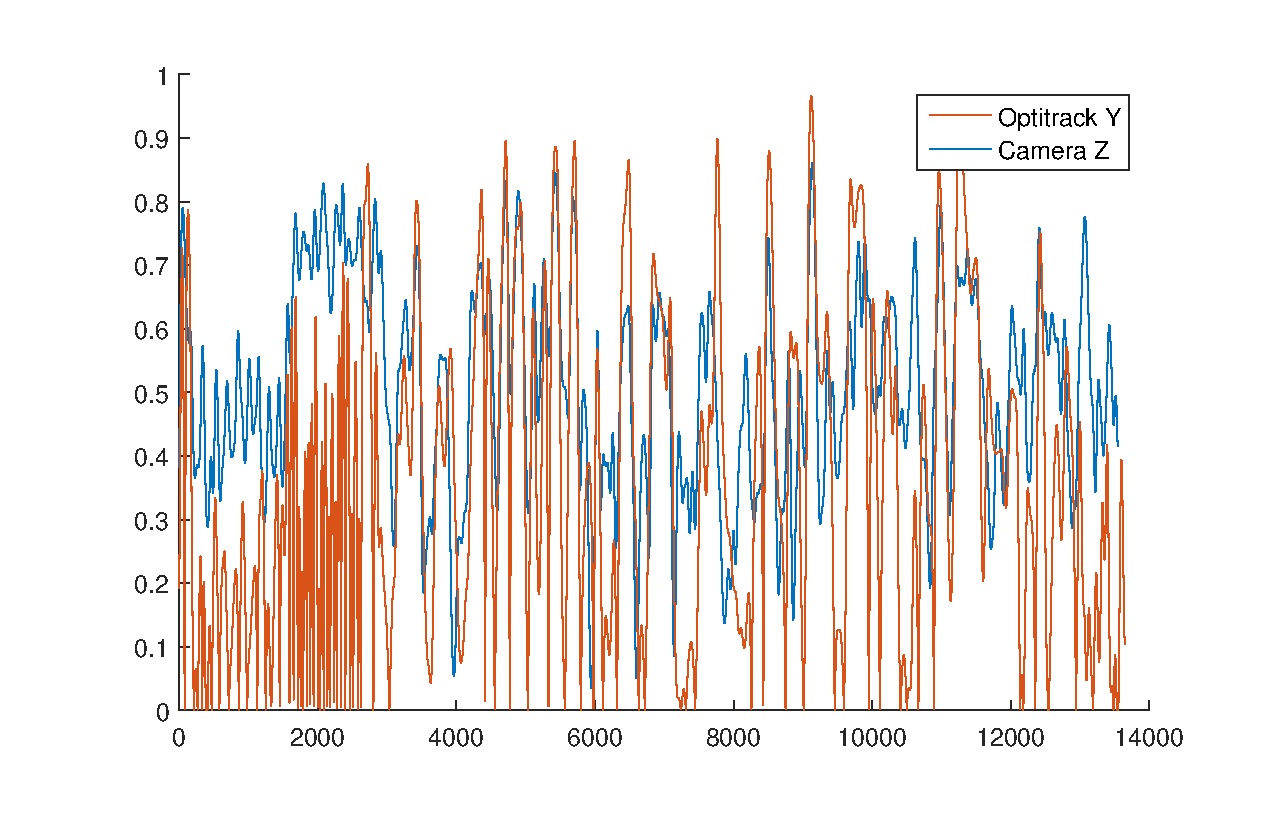
\includegraphics[width = \linewidth]{images/matlab/mocapPos81_sig20}
\caption{\textbf{Comparison of optic-flow sensor estimate with "ground-truth" (cont'd)} - A gaussian window ($\sigma = 20ms$) was applied. The horizontal axis correspond to the index of the frame (~5ms) \label{fig:mocapPos81_sig20}}
\end{figure}

